\usepackage{hyperref}
\usepackage[utf8]{inputenc} % utf8x  defines more symbols, but may cause compatible problems
\usepackage{lmodern,textcomp} % Latin Modern fonts, recognizes euro symbol €

% Math
\usepackage{amssymb}
\usepackage{amsmath}
\usepackage{bm} % bold symbol in math mode
\usepackage{cancel} % https://tex.stackexchange.com/a/75530

% Optional packages
\usepackage{appendixnumberbeamer}
% \usepackage[style=authoryear, backend=bibtex8, natbib=true, maxcitenames=2]{biblatex}
% \usepackage{booktabs}
% \usepackage[scale=2]{ccicons}
% \usepgfplotslibrary{dateplot}
\usepackage{epigraph}
% \usepackage{graphicx}
% \usepackage{import}
\usepackage{multicol}
\usepackage{multirow,array}
% \usepackage{multimedia}
% \usepackage{pgfplots}
\usepackage[super,negative]{nth} % write 1st with superscript
% \usepackage{subcaption} % for subfigure and subtable
\usepackage{tcolorbox}
% \usepackage{ulem} % use the "sout" tag to "strikethrough" text
% \usepackage{xcolor}
\definecolor[named]{darkgreen}{HTML}{008000}
\definecolor{grey}{gray}{0.8}

% -----------------------------------------------------------------------------
% ------NOTES --------------------------------------------------------
% -----------------------------------------------------------------------------
% notes usage: gist.github.com/andrejbauer/ac361549ac2186be0cdb
% pympress viewer: https://github.com/Cimbali/pympress


% -----------------------------------------------------------------------------
% ------ ENVIRONMENT --------------------------------------------------------
% -----------------------------------------------------------------------------

\setcounter{MaxMatrixCols}{10}
\newenvironment{stepenumerate}{\begin{enumerate}[<+->]}{\end{enumerate}}
\newenvironment{stepitemize}{\begin{itemize}[<+->]}{\end{itemize} }
\newenvironment{stepenumeratewithalert}{\begin{enumerate}[<+-| alert@+>]}{\end{enumerate}}
\newenvironment{stepitemizewithalert}{\begin{itemize}[<+-| alert@+>]}{\end{itemize} }
\usetheme[progressbar=frametitle]{Madrid}

% -----------------------------------------------------------------------------
% ------ TITLE AND BIB --------------------------------------------------------
% -----------------------------------------------------------------------------

\title[Green GDP: The Water Environment]{Green GDP}
\subtitle{Valuation of the water environment since 1990}
\author[Thor Donsby Noe]{\textbf{Thor Donsby Noe}\inst{1} \and Jette Bredahl Jacobsen\inst{2}}
\date[23 September 2022]{Labour \& Public Policy Seminar\\
      23 September 2022}
\institute[AU/ECON]{\inst{1}AU/ECON \and \inst{2}UCPH/IFRO}

% \addbibresource{bibliography.bib} % packages, bib, and title page

\setbeamertemplate{navigation symbols}{}

% Select what to do with command \inline{}:
    \newcommand{\inline}[1]{}  % hide inline notes
    % \newcommand{\inline}[1]{\par{\bfseries\color{blue}#1\par}} % show blue inline notes

% Select what to do with command \note{}:
    % \setbeameroption{hide notes} % Only slides
    % \setbeameroption{show only notes} % Only notes
    \setbeameroption{show notes on second screen=right} % Both

\begin{document}

\begin{frame}
    \maketitle
    \footnotesize
    The research project \textit{’Developing and Implementing Green National Accounts and the Green GDP’} is lead by Peter Birch Sørensen (UCPH/ECON) and funded by KR Foundation and the Carlsberg Foundation.
\end{frame}



%%%%%%%%%%%%%%%%%%%%%%%%%%%%%%%%%%%%%%%%%%%%%%%%%%%%%%%%%%%%%%%%%%%%%%%%%%%%%%%%%%%%%%%%%%%%%%%%%%%%%%%%%%%%%%%%%%%%%%%%%%%%%%%%%%%%%%%%%%%%%%%%%%%%%%%%%%%%%%%%%%%%%%%%%%%%%%%%%%%%%%%%%%%%%%%%%%%%%%%%%%%%%%%%%%%%%%%%%%%%%%%%%%%%%%%%%%%%%%%%%%%%%%%%%%%%

\begin{frame}{Outline}
    \tableofcontents
\end{frame}

% \section{Motivation}

\begin{frame}
  GDP has become synonymous with welfare despite its shortcommings.\par
  Our solution: Estimate a Danish \textbf{Green NNP} since 1990.
  \vfill
  \note{
    \textbf{MOTIVATION}\\
    Contrary to Simon Kuznets' warning back in the 1930s where he was in charge of developing the concept of GDP, GDP has largely become synonymous with welfare - which has led to criticism of its shortcomings, and thus, a search for alternative measures.
    \begin{itemize}
      \item The EU Commission motivates their "Beyond GDP initiative" as being "about developing indicators that are as clear and appealing as GDP, but more inclusive of environmental and social aspects of progress. Economic indicators such as GDP were never designed to be comprehensive measures of prosperity and well-being."
    \end{itemize}
    OUR SOLUTION is to estimate a Danish Green GDP since 1990.
    \begin{itemize}
      \item which in the literature is known as the \textbf{Green NNP}.
    \end{itemize}
  }
\end{frame}
\begin{frame}
  GDP has become synonymous with welfare despite its shortcommings.\par
  Our solution: Estimate a Danish \textbf{Green NNP} since 1990.
  \begin{tcolorbox}
    \textbf{RESEARCH FRAMEWORK}
    \begin{align*}
        \text{GNNP} = \text{GDP} &- \text{depreciation of fixed capital assets} \\
        &+ \text{net foreign factor income} \\
        &+ \text{\color{green}benefit of the environmental quality} \\
        &+ \text{\color{green}net growth in the environmental quality}
    \end{align*}
  \end{tcolorbox}
  \vfill
  \note{\textbf{RESEARCH FRAMEWORK}\\
    The Green NNP can be defined like this:\\\bigskip
    (the first part is the) NNP (before accounting for the environment)\\
    +\textcolor{green}{current marginal benefit of the environmental quality} \\
    +\textcolor{green}{present value of net growth in environmental quality}
    \\\bigskip\bigskip
    \textbf{[Only if asked - in more general terms:]}\\\bigskip
    GNNP = NNI\\
    +\textcolor{green}{value of consumption of environmental services} \\
    +\textcolor{green}{value of saving in environmental assets} \\
  }
\end{frame}
\begin{frame}
  GDP has become synonymous with welfare despite its shortcommings.\par
  Our solution: Estimate a Danish \textbf{Green NNP} since 1990.
  \begin{tcolorbox}
    \textbf{RESEARCH FRAMEWORK}
    \begin{align*}
        \text{GNNP} = \text{GDP} &- \text{depreciation of fixed capital assets} \\
        &+ \text{net foreign factor income} \\
        &+ \text{\color{green}benefit of the environmental quality} \\
        &+ \text{\color{green}net growth in the environmental quality}
    \end{align*}
    Contributions are twofold:
    \begin{enumerate}
      \item Impute complete panels of ecological status for 1990-2020.
      \item Shadow prices measured by the marginal current benefit (marginal willingness to pay) using stated preferences.
    \end{enumerate}
  \end{tcolorbox}
  \vfill
  \note{\textbf{CONTRIBUTIONS}\\
    1. \textbf{(...)} for every Danish waterbody
    \begin{itemize}
      \item I.e. for all streams, lakes, fjords, coastal waters and groundwater bodies.
      \item The reason is that data isn't representative but has a systematic overrepresentation of larger waterbodies and those of special concern for the ecological quality.
    \end{itemize}
    2. Apply \textbf{(...)}
  }
\end{frame}
\begin{frame}
  GDP has become synonymous with welfare despite its shortcommings.\par
  Our solution: Estimate a Danish \textbf{Green NNP} since 1990.
  \begin{tcolorbox}
    \textbf{RESEARCH FRAMEWORK}
    \begin{align*}
        \text{GNNP} = \text{GDP} &- \text{depreciation of fixed capital assets} \\
        &+ \text{net foreign factor income} \\
        &+ \text{\color{green}benefit of the environmental quality} \\
        &+ \text{\color{green}net growth in the environmental quality}
    \end{align*}
    Contributions are twofold:
    \begin{enumerate}
      \item Impute complete panels of ecological status for 1990-2020.
      \item Shadow prices measured by the marginal current benefit (marginal willingness to pay) using stated preferences.
    \end{enumerate}
  \end{tcolorbox}
  \textbf{RESULTS AND DISCUSSION}\\
  If $\Delta\text{GNNP}>\Delta\text{NNP}\Rightarrow$ GDP underestimated growth since 1990.
  \note{\textbf{PRELIMINARY RESULTS AND DISCUSSION}\\
    Overall, the quality of ecosystem services has improved since 1990. That is likely to be offset by the costs of GHG emissions and the depletion of exhaustable natural resources\\
    - but if it should turn out that $\Delta\text{GNNP}>\Delta\text{NNP}$
    \begin{itemize}
      \item[$\Rightarrow$] then it would indicate that GDP growth has not been at the expense of the environment.\\\bigskip
    \end{itemize}
    That is, with reservations that we don't fully live up to our international commitment such as the EU Water Framework Directive and the GHG reduction path implied by the Paris Agreement DESPITE outsourcing of our most polluting factories during the period.
  }
\end{frame}
\section{Project overview}

\begin{frame}{Part 1: Panels of ecological status}
  Construct complete panels of ecological status for 1990-2020 comprising every Danish waterbody.\\\bigskip
  Data generating proces:
  \begin{enumerate}
    \item Biologists' field observations with GPS coordinates.
    \item Assign point observations to matching water bodies.
    \item Impute missing observations
    \begin{itemize}
      \item Estimated by \textit{multivariate imputation by chained equations (MICE)} where a \textit{fully conditional specification (FCS)} is constituted by a conditional density for each year.
      \item Physical characteristics are included in a \textit{Bayesian ridge regression} using \textit{iteratively-reweighted regularized least-squares}.
    \end{itemize}
    \item Extrapolation of ecological status of streams for 1990 and 1991.
  \end{enumerate}
  \note{\textit{Our contributions are twofold.}\\\bigskip
    \textbf{CONTRIBUTION 1}\\
    \textbf{(...)} i.e. for all streams, lakes, fjords, coastal waters and groundwater bodies. DGP:
    \begin{enumerate}
      \item ... apply the conservative approach of using the observation that indicates the worst quality.
      \item ... included in the latest Danish waterbody plan.
      \item ... the reason is that data isn't representative but has a systematic overrepresentation of larger waterbodies and those of special concern for the ecological quality.
      \item ... by estimating a linear trend and using it to predict.
    \end{enumerate}
  }
\end{frame}
\begin{frame}{Contribution 2: Apply valuation studies}
  Shadow prices measured by the marginal current benefits of improving the quality of the Danish water environment on a national level.\\\bigskip
  I.e. the marginal willingness to pay using stated preference studies:
  \begin{itemize}
    \item \textbf{Surface waters}: Meta regressions analysis of 32 nordic studies (Zandersen et al, \textit{pending}, DCE Technical Note).
    \item \textbf{Ground water:} \textit{Choice experiment} with only 383 respondents around Limfjorden with overrepresentation of women and higher educated (Larsen et al, 2020, IFRO Working Paper).
  \end{itemize}
  \note{\textbf{CONTRIBUTION 2}\\
  }
\end{frame}
\section{Examples of stated preferences}

\begin{frame}{Example 1: Characteristics of ground water quality}
  \center
  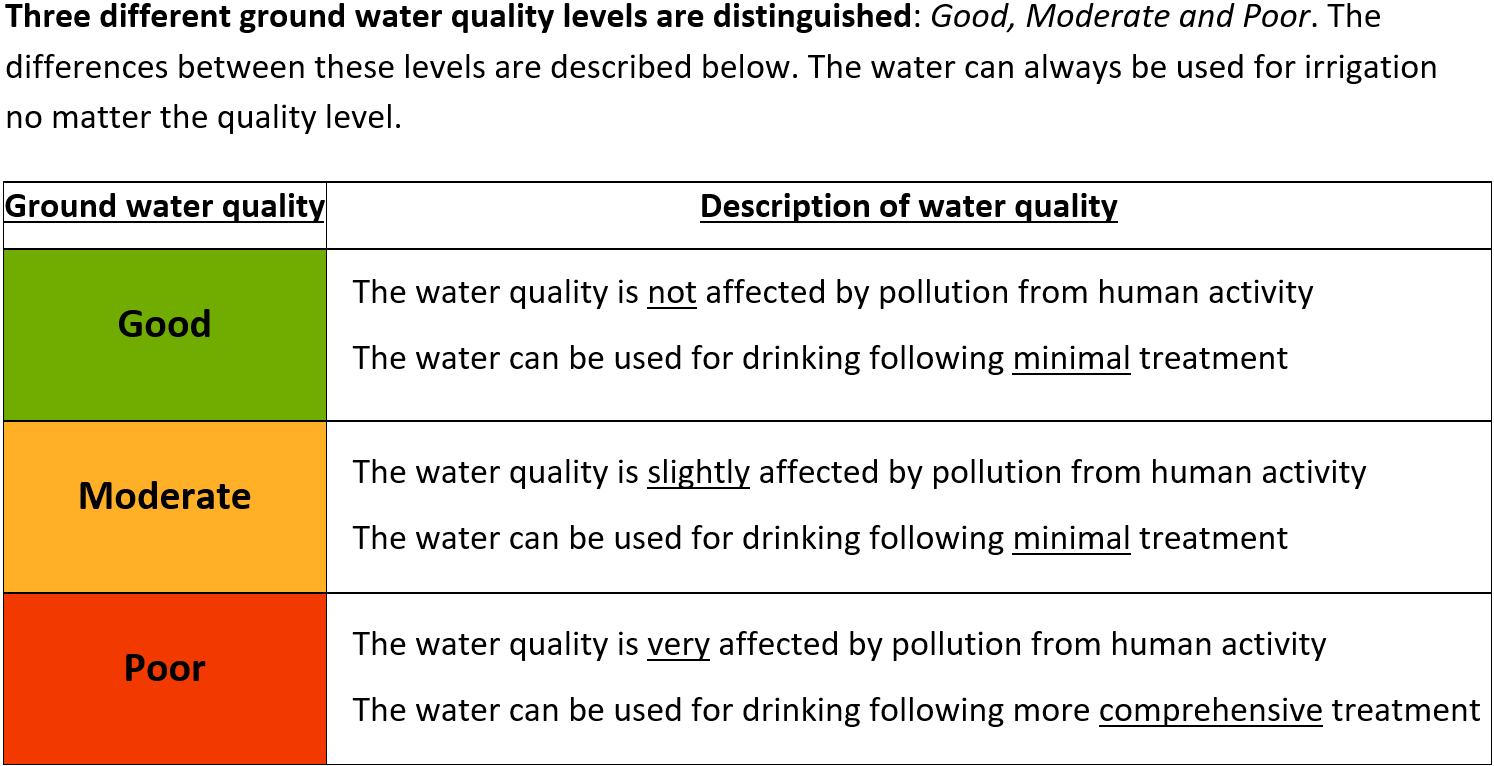
\includegraphics[width=\textwidth]{figures/IFRO_WP_characteristic_groundwater}
  \note{\textbf{EXAMPLE 1:}\\
    Description of the expected ground water quality following different policy proposals.
  }
\end{frame}

\begin{frame}{Example 2: Choice set for ground water quality}
  \center
  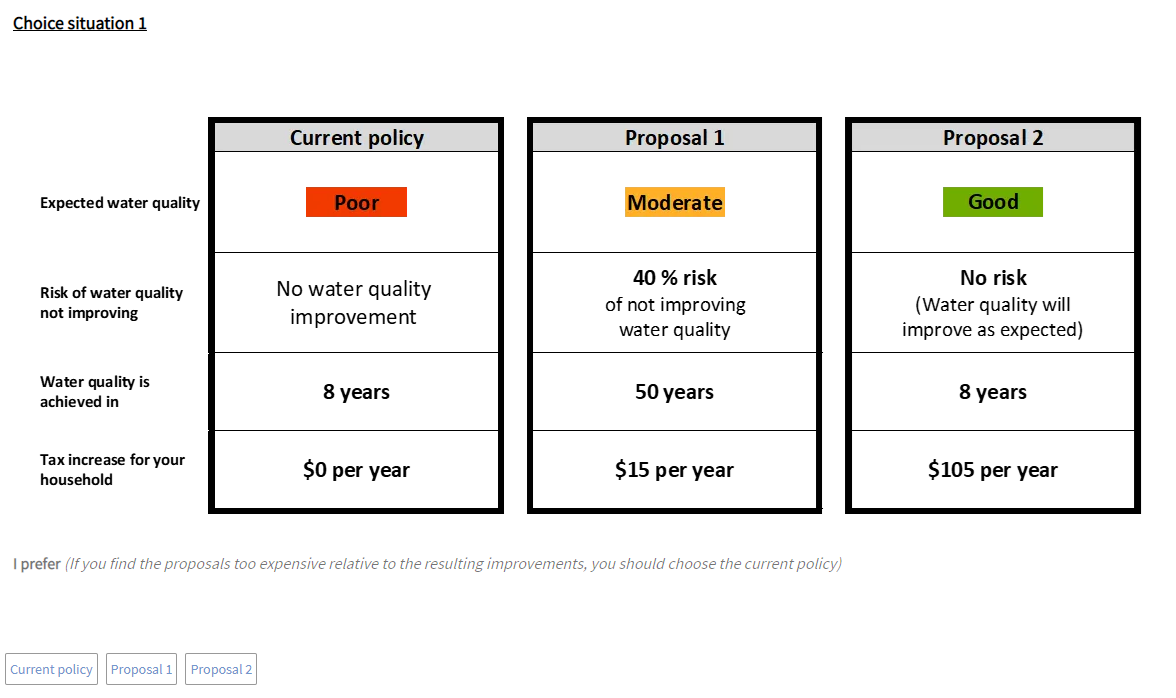
\includegraphics[width=\textwidth]{figures/IFRO_WP_choice_groundwater}
  \note{\textbf{EXAMPLE 2:}\\
    Marginal willingness to pay per household is deduced from elaborate questionnaires such as the one containing this choice set regarding different proposet policies to improve ground water quality.
  }
\end{frame}
\section{Preliminary results and discussion}

\begin{frame}{Preliminary results and discussion}
  The quality of ecosystem services has improved from 1990-2020.\\\bigskip
  If $\Delta\text{GNNP}>\Delta\text{NNP}\Rightarrow$ GDP underestimated growth since 1990.\\\bigskip
  \vfill
  \note{\textbf{PRELIMINARY RESULTS AND DISCUSSION}\\
    Overall, the quality of ecosystem services has improved since 1990. That is likely to be offset by the costs of GHG emissions and the depletion of exhaustable natural resources\\
    - but if it should turn out that $\Delta\text{GNNP}>\Delta\text{NNP}$,
    \begin{itemize}
      \item[$\Rightarrow$] then it would indicate that GDP growth has not been at the expense of the environment according to the definition of "strong" sustainability.\\\bigskip
    \end{itemize}
    That is, with reservations that we don't fully live up to our international commitment such as the EU Water Framework Directive and the GHG reduction path implied by the Paris Agreement DESPITE outsourcing of our most polluting factories during the period.
  }
\end{frame}
\begin{frame}{Preliminary results and discussion}
  The quality of ecosystem services has improved from 1990-2020.\\\bigskip
  If $\Delta\text{GNNP}>\Delta\text{NNP}\Rightarrow$ GDP underestimated growth since 1990.\\\bigskip
  \textit{Comprehensive robustness checks are necessary.}
  \note{\textbf{ROBUSTNESS}\\
    To construct an unbroken time series, we need to only rely on test methods for ecological and chemical quality that has been applied since the early 90s while applying so-called "heroic assumptions", thus
    \begin{itemize}
      \item[$\Rightarrow$] \textit{Comprehensive robustness checks are necessary}
    \end{itemize}
    some of which will have to be "back-of-the-envelope" calculations.
  }
\end{frame}

\end{document}